\documentclass[10pt,a4paper]{article}  % Changed from 12pt to 10pt

% Add geometry package for margin control
\usepackage[left=2.5cm,right=2.5cm,top=1.5cm,bottom=2.5cm]{geometry}

% Packages
\usepackage[utf8]{inputenc}
\usepackage{graphicx}
\usepackage{amsmath}
\usepackage{hyperref}
\usepackage{listings}
\usepackage{xcolor}

% Configure code listings
\definecolor{codegreen}{rgb}{0,0.6,0}
\definecolor{codegray}{rgb}{0.5,0.5,0.5}
\definecolor{codepurple}{rgb}{0.58,0,0.82}
\definecolor{backcolour}{rgb}{0.95,0.95,0.92}

\lstdefinestyle{mystyle}{
    backgroundcolor=\color{backcolour},   
    commentstyle=\color{codegreen},
    keywordstyle=\color{magenta},
    numberstyle=\tiny\color{codegray},
    stringstyle=\color{codepurple},
    basicstyle=\ttfamily\footnotesize,
    breakatwhitespace=false,         
    breaklines=true,                 
    captionpos=b,                    
    keepspaces=true,                 
    numbers=left,                    
    numbersep=5pt,                  
    showspaces=false,                
    showstringspaces=false,
    showtabs=false,                  
    tabsize=2
}

\lstset{style=mystyle}

% Title and author information
\title{COP290 C lab: Spreadsheet Implementation}
\author{Shivankur Gupta 2023CS10809\\ Vanshika 2023CS10746\\ Samyak Sanghvi 2023CS10807}

\begin{document}

\maketitle



\tableofcontents

\section{Introduction}
In this implementation of Spreadsheet, we have modeled the problem to be a directed acyclic graph. In order to ensure that the formulas are valid and conserved against individual cell value change, we have used topo sort and stacks to efficiently find the order of recalculation and manage dependencies upon changing the value of a cell.

\section{Data Structures and Uses}
The following Datastrutures have been used in this implementation

\begin{itemize}
    \item \textbf{Ordered Set (AVL Tree)}: To store the list of dependencies of a cell.
    \item \textbf{Cell Structure}: To store the value, formula, location and dependents of a cell.
    \item \textbf{Directed Acyclic Graph}: To model and capture formula dependencies.
    \item \textbf{Linked List}: To store the order of operations after Topo sort.
    \item \textbf{Stack}: To replace recursion, allowing larger recursion depths.
    \item \textbf{Vector}: To initially store the list of dependencies of a cell.
\end{itemize}



\section{Design Decisions}
The following design decisions have been made in the implementation of the spreadsheet:
\subsection{Cell Struct}
The Cell struct is a fundamental data structure in our implementation that represents each cell in the spreadsheet. It contains the following components:

\begin{itemize}
    \item \textbf{row, col}: Integer values storing the location coordinates of the cell in the spreadsheet
    \item \textbf{value}: Stores the numerical value of the cell
    \item \textbf{error}: A flag indicating invalid arithmetic operations 
    \item \textbf{formula}: A character pointer storing the formula string used to calculate the cell's value
    \item \textbf{dependents}: A union of a Vector and an ordered set (implemented as an AVL tree) that store references to all cells that use this cell in their formulas
    
\end{itemize}


\noindent{The design ensures that each cell can maintain exactly one formula, which is consistent with spreadsheet functionality. The dependents list is crucial for efficient updates when a cell's value changes, as it allows us to identify and recalculate all affected cells in the correct order.\\}


\noindent{A vector has the most efficient space management, but extraction will take time in a vector, so for the first few commands (up to 3 dependencies),%edit here% 
we store them in a vector. When the number of dependencies increases, we store the move and free the vector, and store them in an ordered set. This ensures that the performance is at par while increasing space optimization for the first few commands.}

\subsection{OrderedSet Implementation}
For efficiently storing the list of dependents for each cell, we evaluated two primary data structure options:

\begin{itemize}
    \item \textbf{AVL Tree}: This self-balancing binary search tree ensures efficient space utilization with a time complexity of O(log n) for operations. Given that n is at most of order $10^8$ in our implementation, the logarithmic time complexity does not significantly impact performance.
    
    \item \textbf{Hash Table}: While offering amortized O(1) time complexity, this option presented challenges:
    \begin{itemize}
        \item Difficulty in designing a conflict-free hash function due to the repetitive nature of cell names
        \item Higher space requirements compared to the AVL tree implementation
    \end{itemize}
\end{itemize}

We chose to implement the OrderedSet using an AVL tree structure, prioritizing space efficiency and reliable performance characteristics over raw speed.

\subsection{Dependency Management}
Our dependency management system incorporates several key components:

\begin{itemize}
    \item \textbf{Directed Acyclic Graph (DAG)}: We implemented a DAG structure to model cell dependencies, allowing us to efficiently track relationships between cells and detect circular dependencies.
    
    \item \textbf{Topological Sort}: We employed a topological sort algorithm to determine the correct order of cell recalculations, ensuring that all dependencies are resolved before computing dependent cell values.
    
    \item \textbf{Linked List Implementation}: To store the sequential output from the topological sort, we used a linked list data structure. This provides efficient traversal of the calculation order while maintaining the exact sequence of operations.
    
    \item \textbf{Custom Stack}: To handle deep dependency chains without encountering stack overflow issues, we implemented a custom stack data structure that replaces recursive calls. This allows our implementation to handle larger spreadsheets with complex dependency relationships.
\end{itemize}

\begin{figure}[h!]
    \centering
    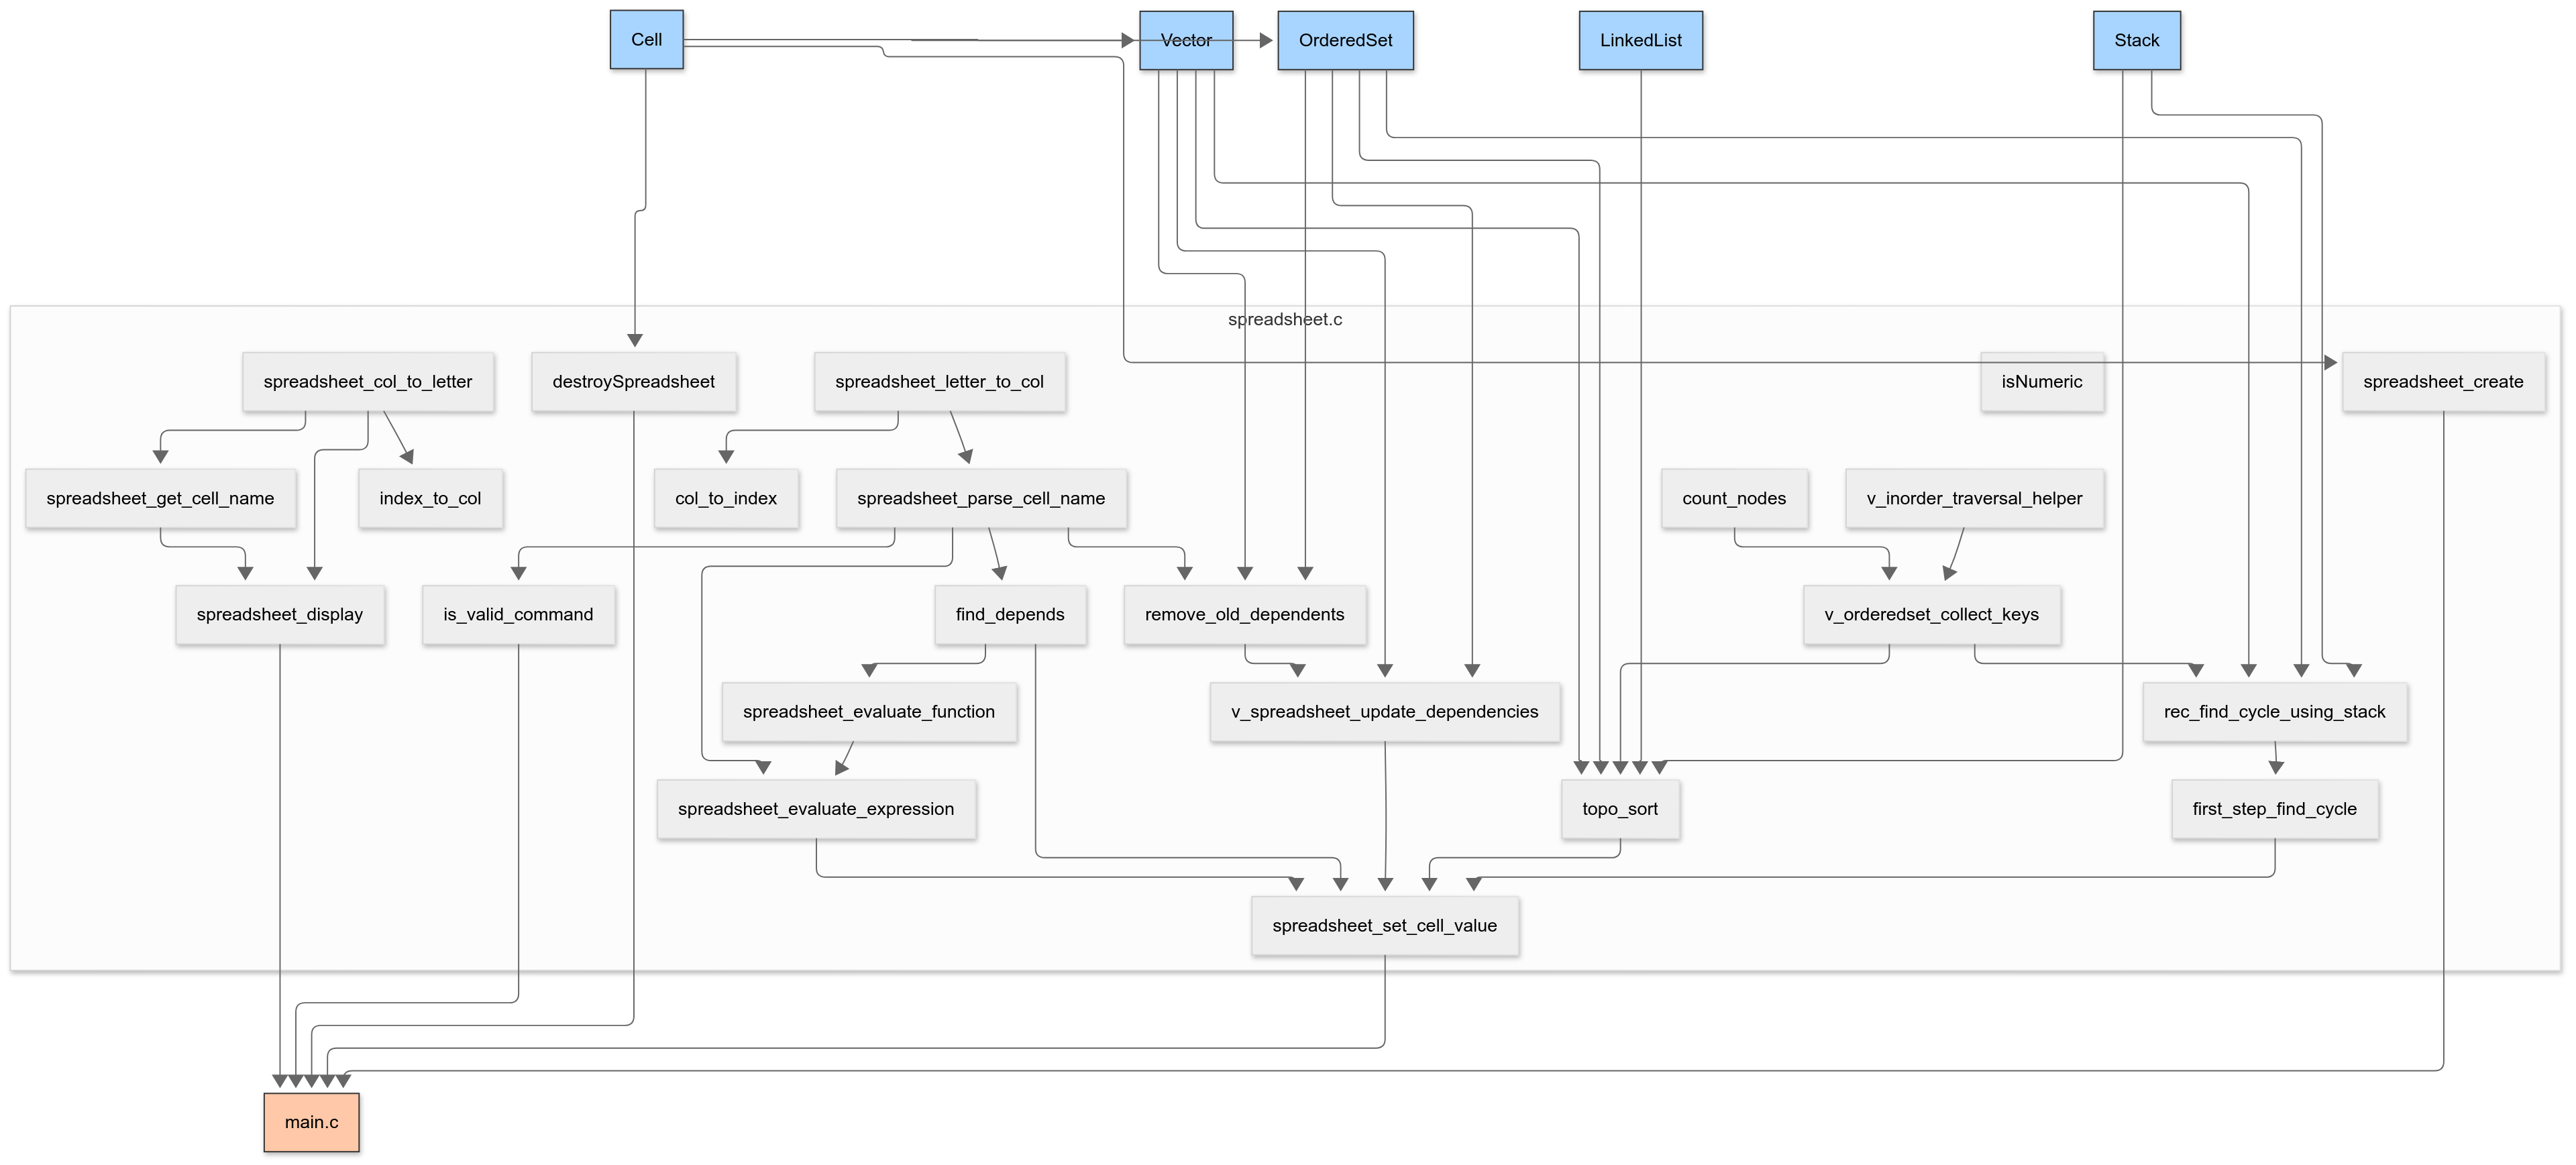
\includegraphics[width=0.8\textwidth]{sysarch.png}
    \caption{This is the overview of system architecture}
    \label{fig:system_architecture}
\end{figure}

\section{Covered Edge Cases}

In our testing suite, we have done unit testing as well as Blackbox testing.
The following edge cases were covered:

\begin{itemize}
    \item \textbf{Cyclic Dependency}: We tested if the system can detect cyclic dependencies between cells. The system correctly identifies circular dependencies and raises an error message while rejecting the formula. (tested by \texttt{input\_cycle.txt} and \texttt{spreadsheet\_test.c}).
    \item \textbf{Invalid Formula}: In addition to the well-defined signatures, we have given support for categorizing numerals with \(+\) and \(-\) signs, so inputs like \(1++1\) and \(1+-1\) are considered valid. All other inputs and out-of-bound inputs are raised as invalid. We do not support case invariance in any function or arbitrary '0's in the cell names. (tested by \texttt{input\_arbit.txt}, \texttt{input\_unrec\_cmds.txt} and \texttt{spreadsheet\_test.c}).
    \item \textbf{Sleep Cells}: We tested if the normal sleep function works as expected. We tested for cascaded sleep cells and their behavior upon changing the base of the cascade. We also tested for SLEEP(num), where num is a negative number. (tested by \texttt{input\_sleep.txt} and \texttt{spreadsheet\_test.c}).
    \item \textbf{Invalid Arithmeic}: We tested if logically invalid arithmetic operations, such as division by zero, and its cascades are flagged correctly by showing ERR on display. (tested by \texttt{input\_checks\_err.txt})
    \item \textbf{Scrolling}: We unit-tested the scrolling nature to match the specifications of the assignment. (tested by \texttt{scroll\_test.c})
    \item \textbf{Datastructures Correctness}: We unit-tested for the correctness and robustness of AVL tree, Linked List, Cell struct and Stack. (tested by \texttt{orderedset\_test.c}, \texttt{linked\_list\_test.c}, \texttt{cell\_test.c} and \texttt{stack\_test.c})
\end{itemize}

\section{Performance}
After 



% \section{References}






\end{document}
